\newpage
\section{柔軟外皮を備えたワイヤ駆動式魚ロボットの開発}
\subsection{本研究の目的}
前章で述べたように,先行研究\cite{kyu}では屈曲可能な胴体を持ち,柔軟外皮を装着して完全防水を可能にした魚ロボットの開発に成功した.しかし,リンクと外皮に隙間ができてしまい,
リンクの動きを外皮にうまく伝えることができなかった.そこで本研究では魚らしいしなやかな動きを可能にするワイヤ駆動式の魚ロボットをベースにリンクに外皮を追従させ,尾びれのみならず
胴体部まで振って泳ぐことが可能なロボットの開発を目指す.さらに外皮の有無による遊泳性能の向上の変化について実機実験によって検証する.

\subsection{ワイヤ駆動式魚型ロボットの動作原理}
昨年度卒業研究で提案され,本研究でも採用したワイヤ駆動の動作原理を記す.ロボット前方にはプーリを取り付けたサーボモータを配置し,胴体部には弾性体とそれに固定した骨格リンクを配置する.
ワイヤはプーリーから骨格リンクに設けられた穴を通って尾びれ付け根まで伸びており,プーリーを回してワイヤを巻き取ることによって弾性体が曲がり,胴体部を屈曲させることができる.それを左
右に繰り返すことで遊泳を可能にする(図\ref{fig:waiyakudou})

\begin{figure}[b]
   \centering
   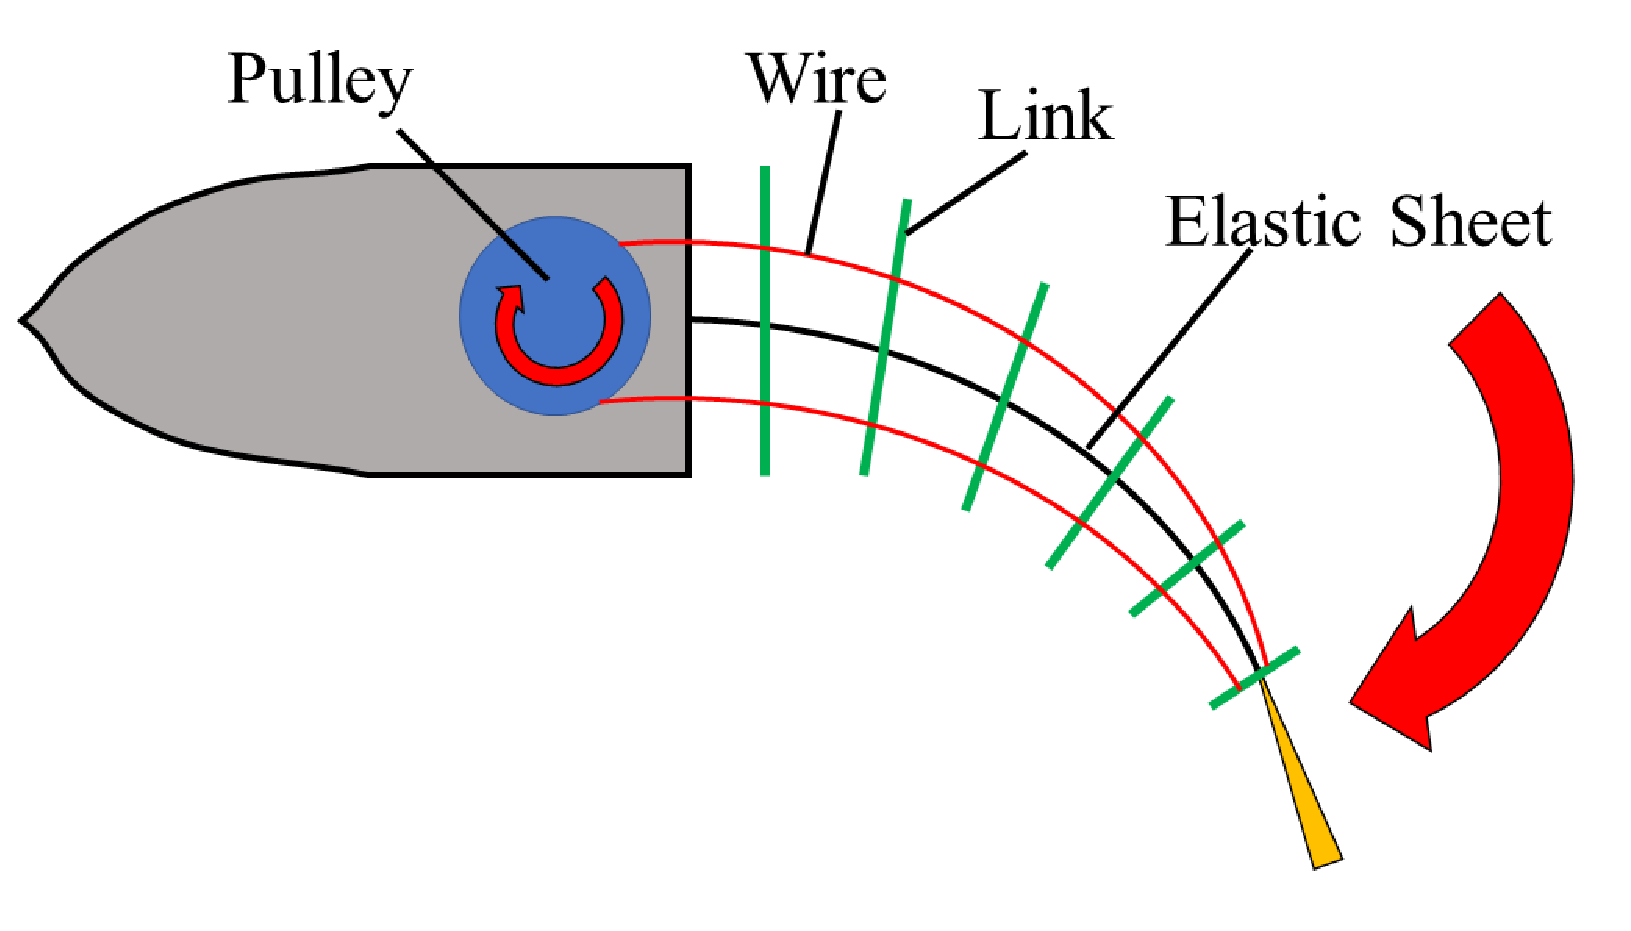
\includegraphics[width=0.6\linewidth]{chapters/picture/waiyakudou.eps}
   \caption{ワイヤ駆動のイメージ}
   \label{fig:waiyakudou}
\end{figure}

\subsection{試作機}
\subsubsection{試作機の作製}
まず,昨年度卒業研究を参考にして試作機を作製した.図\ref{fig:sisaku}に外観を,図\ref{fig:kouzou_sisaku}に構造を示す.全長は530 mm,重量は478 gである.試作機は頭部と胴体部の二つ
の部分で構成している.

頭部には制御回路とバッテリーを搭載しており,えらにあたる部分には防水仕様(IP67)の サーボモータ(Flash Hobby, M45CHW)を配置している.使用マイコンはM5Stamp Pico(M5Stack Technology 社),
使用バッテリーはマイコン用の3.7 V,サーボモータ用の7.4 Vの二つのLi-ionバッテリーを使用している.そのため,頭部は防水が必要となり,頭部の断面にOリングをはめ込むことによって防水を行っている.
頭部はネジ穴が空いたものと,ナット用の穴が空いたものに分かれており,これらはM1.7ネジで固定される.
胴体部は骨格リンク(PLA樹脂)と弾性体(ポリプロピレン板,厚さ0.75 mm),尾びれ(TPU樹脂,厚さ2 mm)で構成されており,骨格リンクは図のように楕円形にして作製し,ワイヤ(ポリエステル製,0.40 mm)
を通す穴を空けている.

\begin{figure}[t]
    \centering
    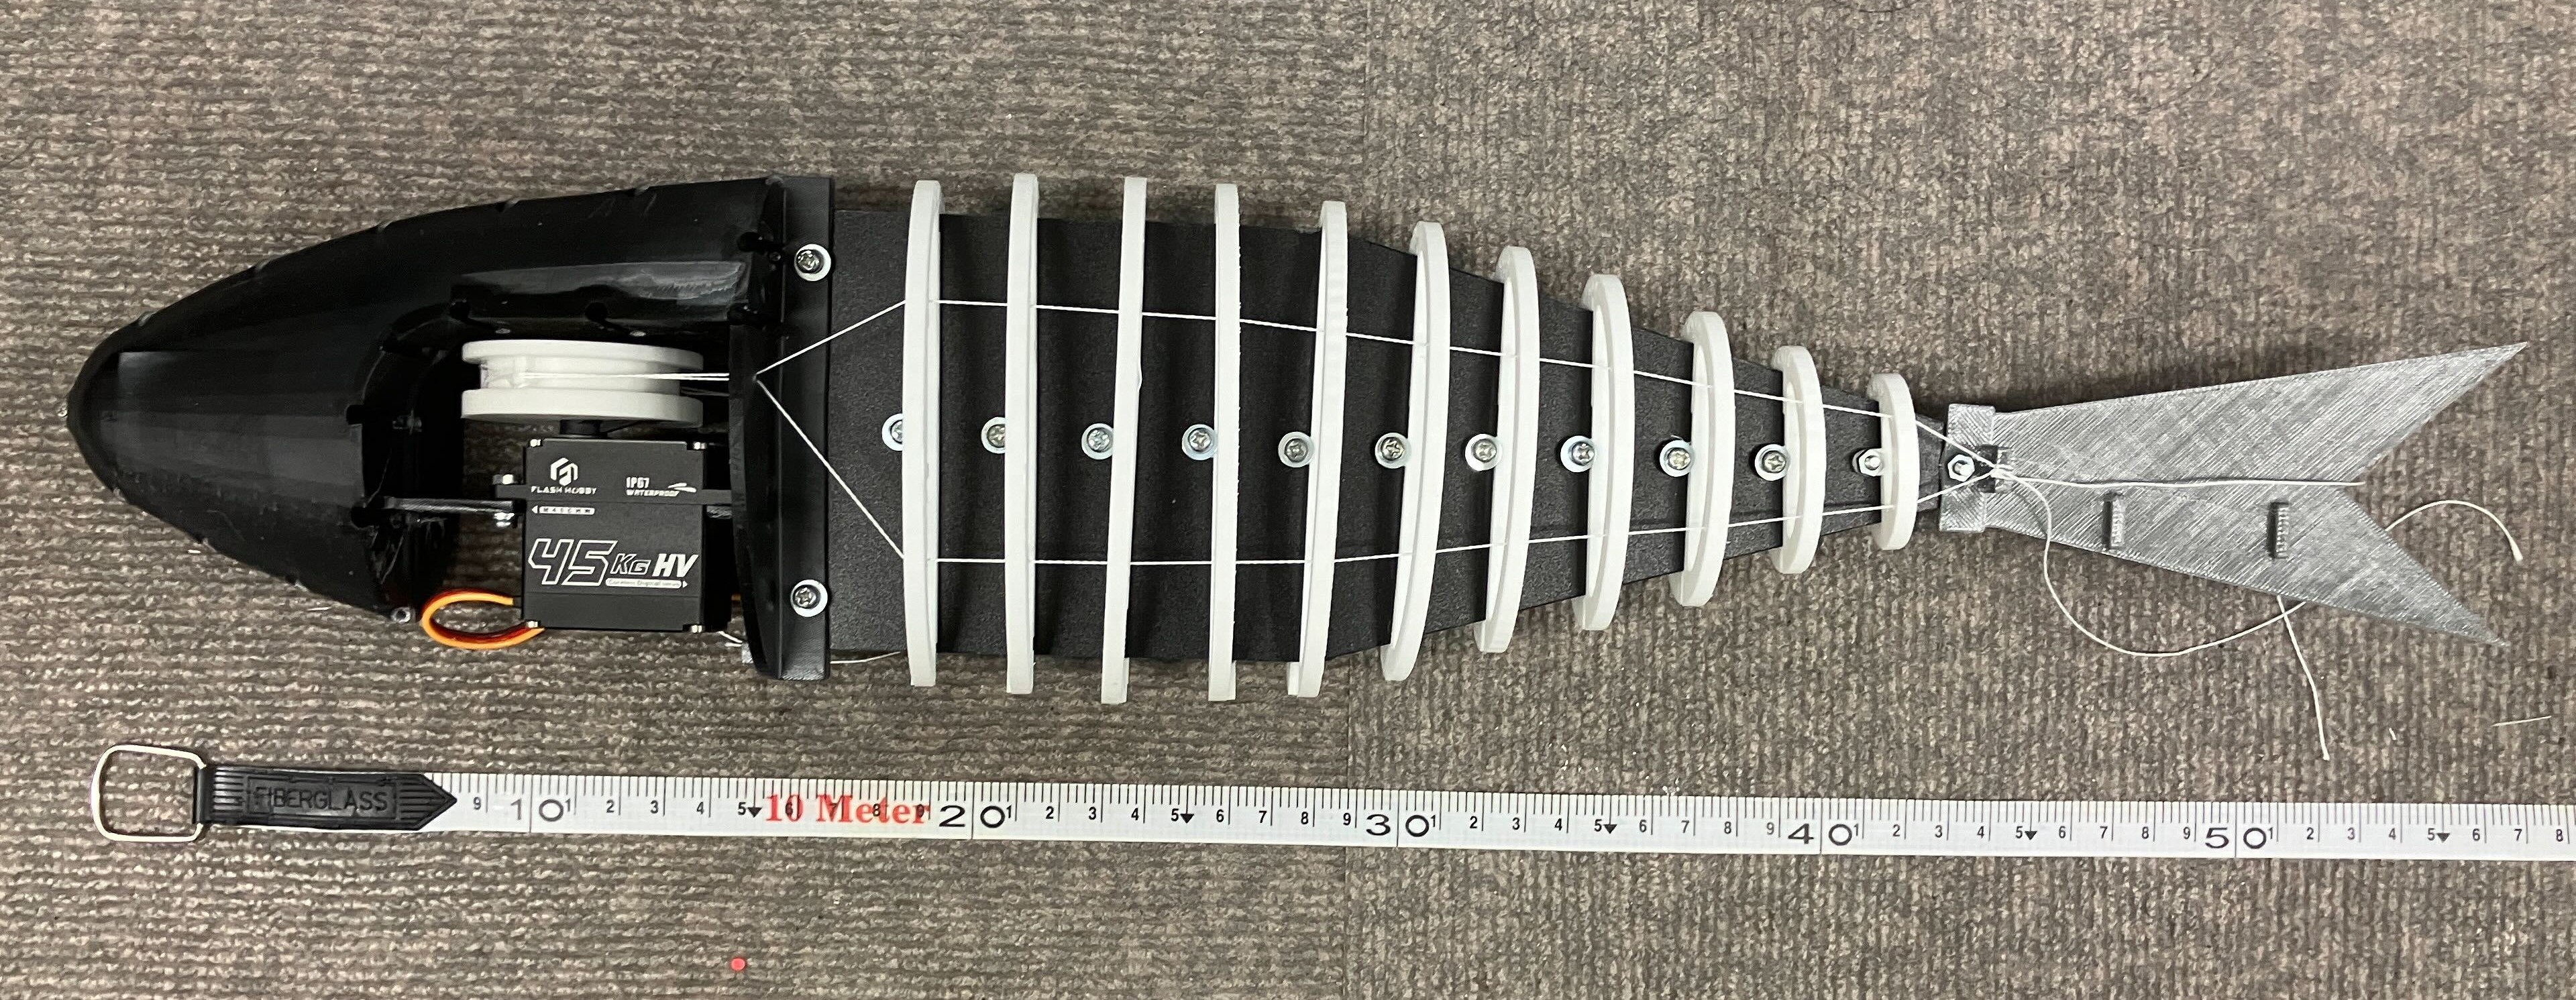
\includegraphics[width=0.80\linewidth]{chapters/picture/sisaku.jpg}
    \caption{試作機の外観}
    \label{fig:sisaku}
\end{figure}
\begin{figure}[t]
    \centering
    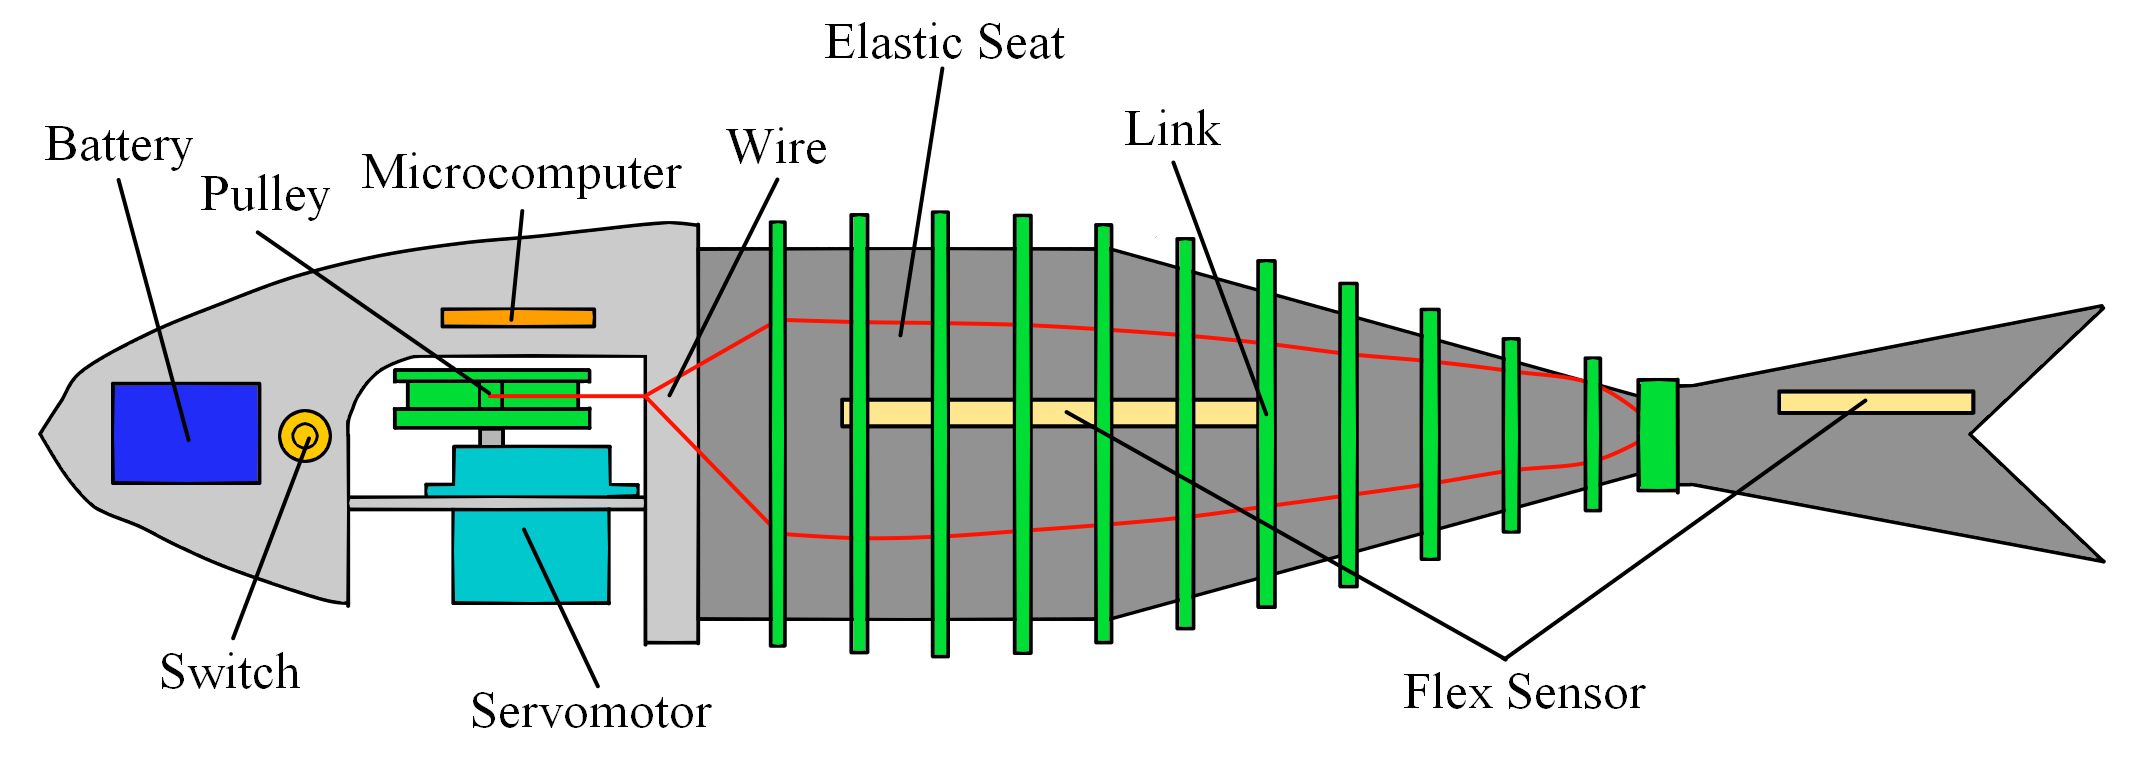
\includegraphics[width=0.80\linewidth]{chapters/picture/tentativeschematic.png}
    \caption{試作機の構造}
    \label{fig:kouzou_sisaku}
\end{figure}
\begin{figure}[t]
    \centering
     \begin{minipage}[b]{0.50\linewidth}
        \centering
        \setPicture{ring.jpg}
        \caption{頭部断面のようす}
        \label{fig:danmen}
     \end{minipage}
     \hspace{0.05\linewidth}
     \begin{minipage}[b]{0.25\linewidth}
        \centering
        \setPicture{jikkilink.png}
        \caption{骨格リンク}
        \label{fig:link_sen}
     \end{minipage}
\end{figure}

\subsubsection{防水テスト・遊泳テスト}
機体完成後,防水テストと遊泳テストを行った.まず防水テストは水没すると赤くなるシールを頭部内部に貼り,水深120 mmの水槽で2 分間沈める防水テストを7回行った.

\begin{figure}[t]
    \centering
    \setPicture{sisakuoyogu2.png}
    \caption{遊泳テストの様子}
    \label{fig:test_sisaku}
\end{figure}
\begin{figure}[t]
    \centering
    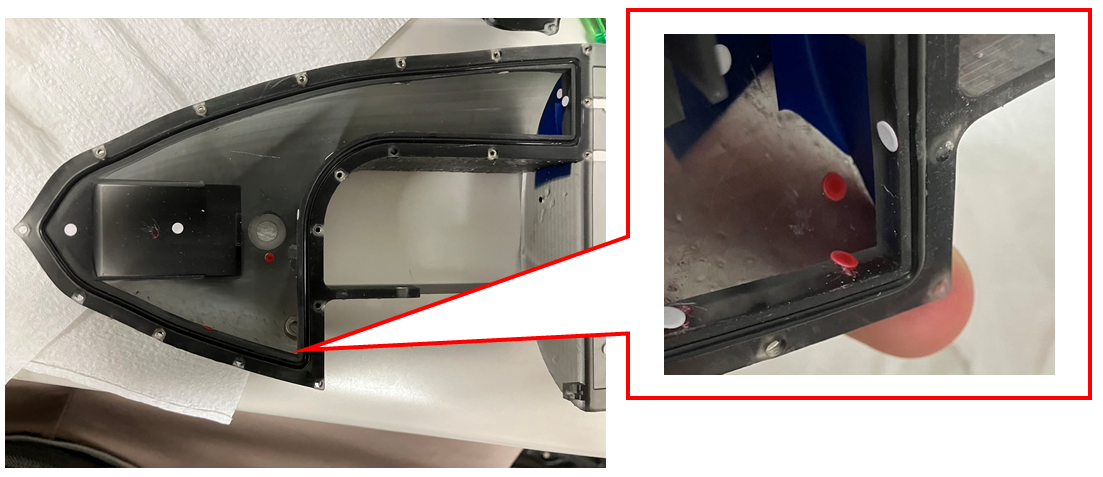
\includegraphics[width=0.80\linewidth]{chapters/picture/bousuitest.png}
    \caption{頭部下方浸水のようす}
    \label{fig:bousuitest_sisaku}
\end{figure}

\subsubsection{試作機から得られた知見}
試作機の作製・動作確認を通して得られたこととして,まず頭部をネジとOリングを用いて防水する方法は限度があることが分かった.試作機には防水箇所確認のため水没すると
赤くなるシールを貼っており,推進120 mmの水槽で2 分間沈める防水実験を7回行った.しかし,ネジの締め方や締め具合を何度か調整しても図のように頭部下方は赤くなる,
つまり浸水してしまい,完全な防水機能を有することはできていなかった.また,頭部を固定するネジが多いと,バッテリー交換がしにくく,メンテナンス性が
悪くなるということも分かった.以上のことから防水方法を変更し,メンテナンス性を向上させた頭部に改良することが必要だとわかった.

\newpage

\subsection{ワイヤ駆動式柔軟外皮装着型魚ロボットの開発}
ここからは本研究で開発した機体について述べる.
図\ref{fig:gaikan}に開発した機体の外観を,図\ref{fig:kouzou}に構造を示す.開発した魚ロボットは体長470 mm,重量は重りを含めて710 gである.ロボットの外形は
先行研究において作製されたアジのモデルデータをもとに作製し,サイズは2倍とした.本機体は頭部・胴体部・外皮の3つからなり,頭部と胴体部をそれぞれ別の柔軟外皮で包む
構造になっている.また,頭部は防水区画とし,胴体部は水中姿勢を水平にするために浸水させた.

\begin{figure}[htbp]
    \centering  
    \begin{subfigure}[b]{0.9\linewidth}
        \centering
        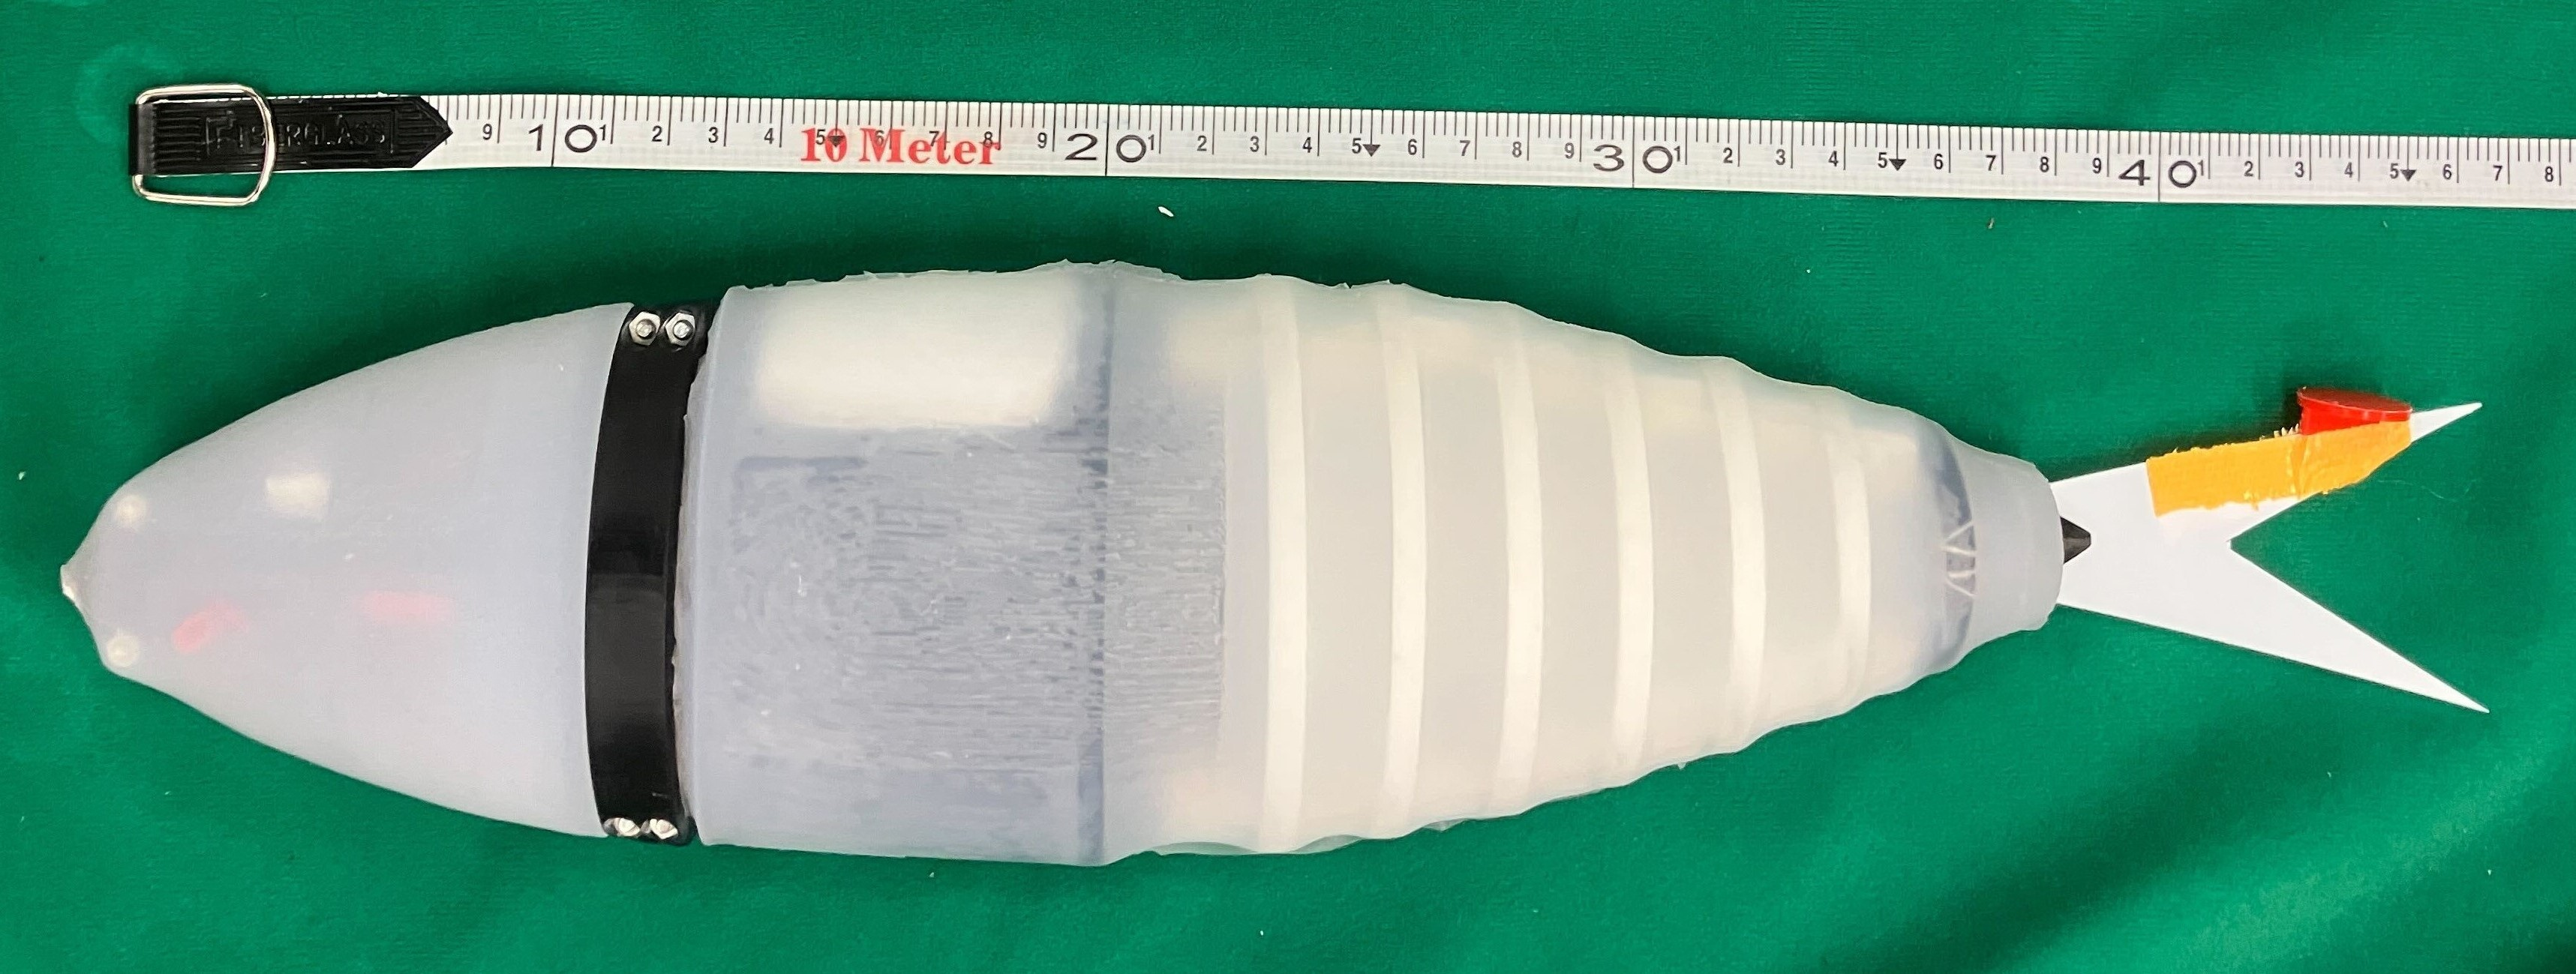
\includegraphics[width=0.9\linewidth]{chapters/picture/withskin.jpg}
        \subcaption{外皮あり}
        \label{fig:fishrobo_with}
    \end{subfigure}
    \begin{subfigure}[b]{0.9\linewidth}
        \centering
        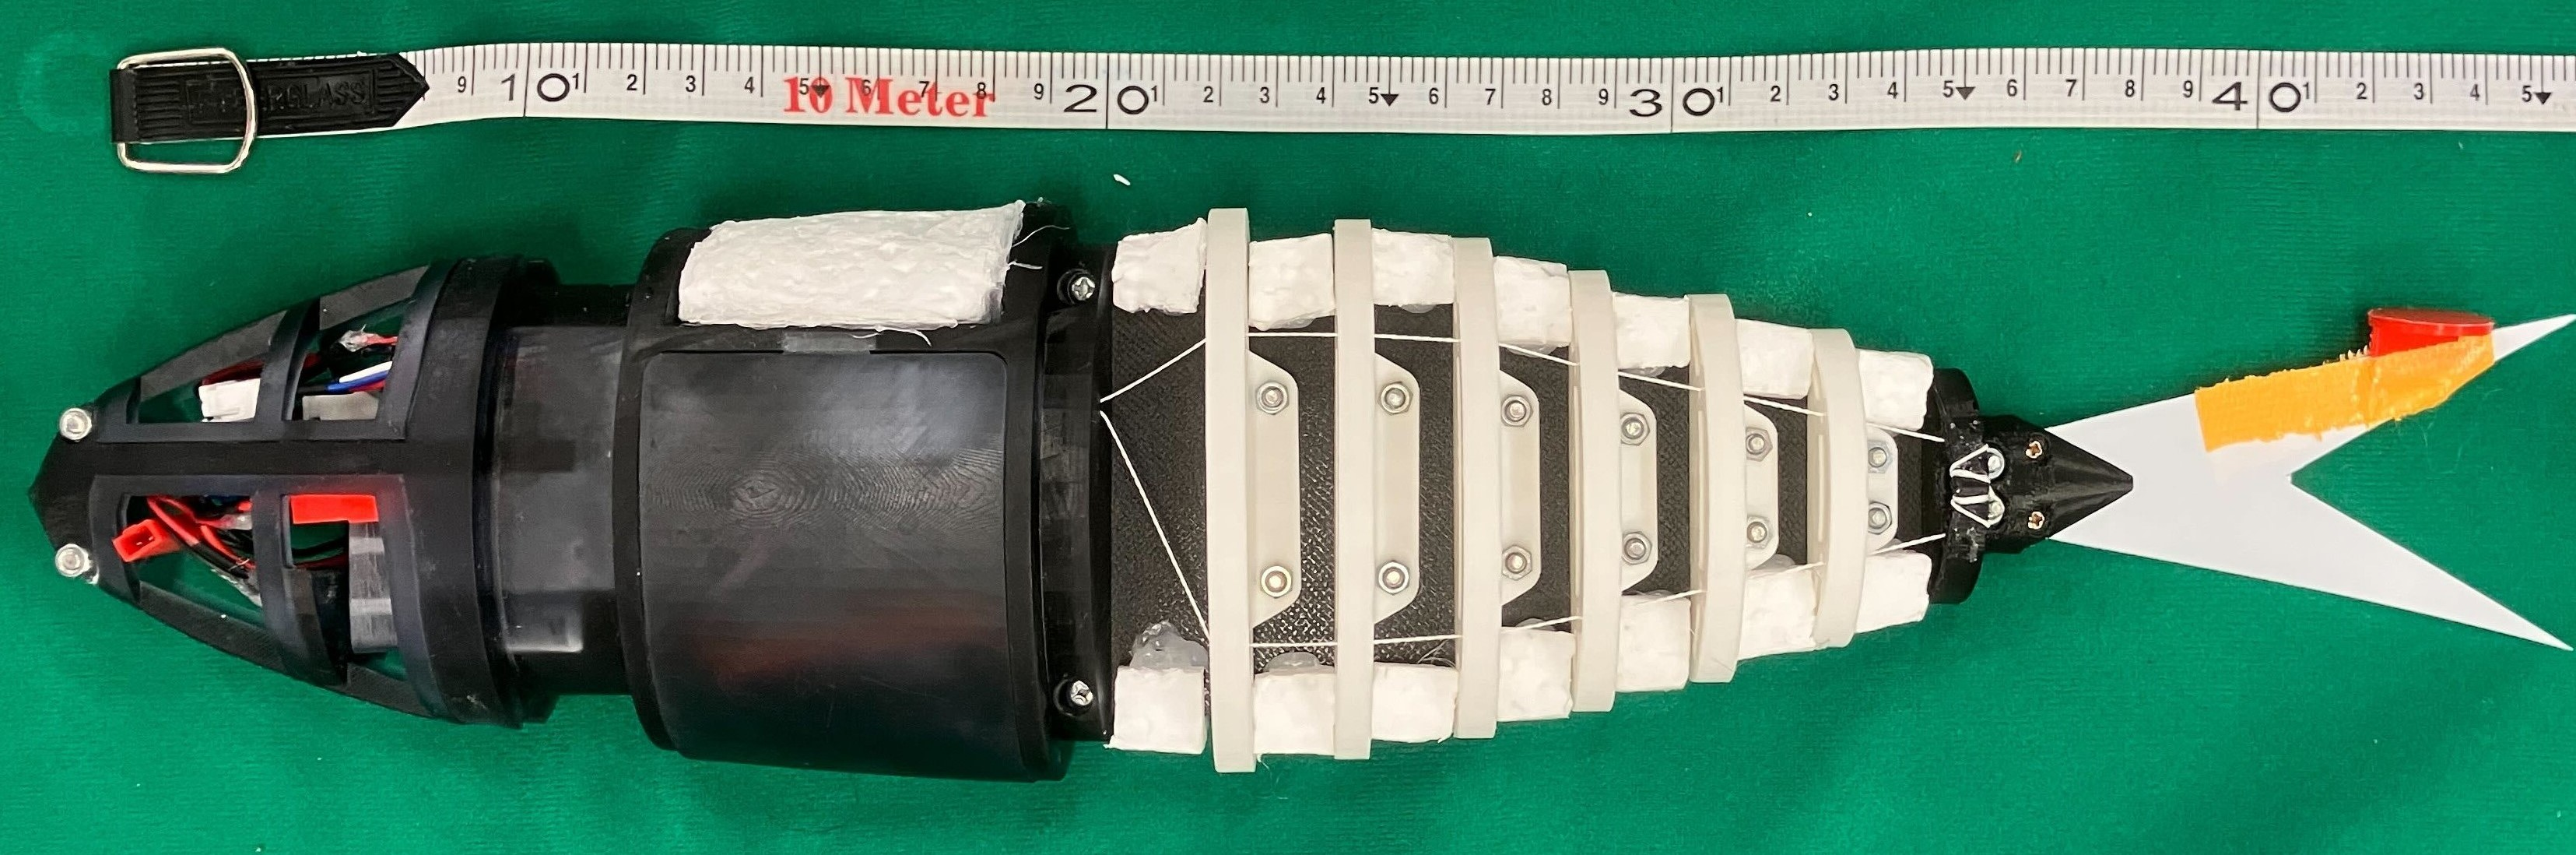
\includegraphics[width=0.9\linewidth]{chapters/picture/skinless.jpg}
        \subcaption{外皮なし}
        \label{fig:fishrobo_less}
    \end{subfigure}
    \begin{subfigure}[b]{0.9\linewidth}
        \centering
        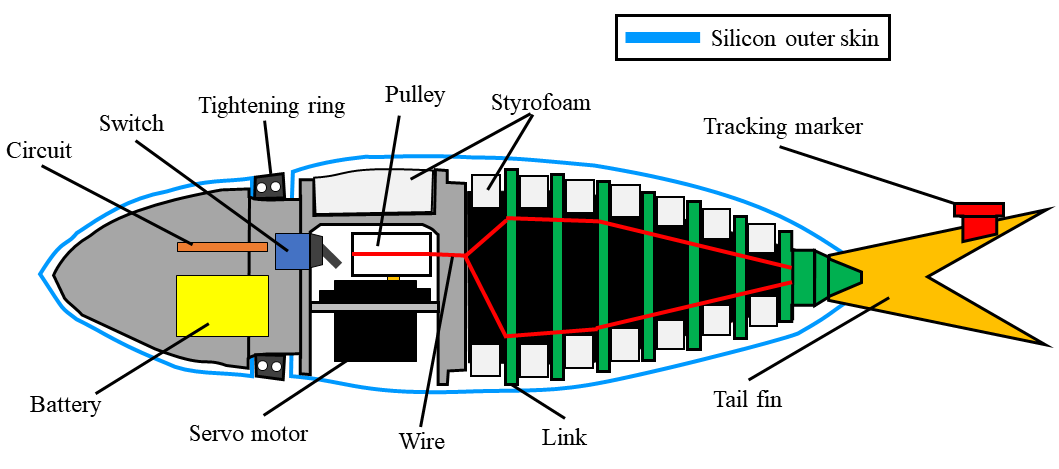
\includegraphics[width=0.9\linewidth]{chapters/picture/fish.png}
        \caption{開発したロボットの構造}
        \label{fig:kouzou}
    \end{subfigure}
    \caption{開発したロボット}
    \label{fig:gaikan}
\end{figure}

\subsubsection{頭部}
頭部は光造形方式の3Dプリンタで作製しており,胴体前部と一体となっている.内部にはバッテリーと制御回路を搭載しており,使用するバッテリー,マイコン共に試作機から変更はしていない.バッテリーとマイコンを
搭載する都合上頭部を防水する必要があり,試作機から得た知見をもとに今回はOリングによる防水ではなく,シリコン製の外皮を用いて防水を行った.

防水方法としてはシリコン製の外皮を頭部にかぶせ,根元を防水リングによって締め付けることで防水を行う(図\ref{fig:bousui}).防水リングのサイズはをもとに締め付ける部分が短径,長径ともに10%つぶ
せるように設計した.また,試作機と同様に防水実験を1回行ったが,内部に貼ったシールはどれも赤く染まらず,完全な防水ができた(図\ref{fig:bousui_test}).

\begin{figure}[htpb]
    \centering
    \begin{tabular}{cc}
        \begin{minipage}[b]{0.43\linewidth}
            \centering
            \setPicture{bousui.pdf}
            \subcaption{防水構造}
            \label{fig:bousui_kouzou} 
        \end{minipage}
        \begin{minipage}[b]{0.43\linewidth}
            \centering
            \setPicture{jissai.jpg}
            \subcaption{実際の様子}
            \label{fig:bousui_jissai} 
        \end{minipage}
    \end{tabular}
    \caption{頭部防水について}
    \label{fig:bousui}
\end{figure}
\begin{figure}[htbp]
    \centering
    \begin{tabular}{ccc}
        \begin{minipage}[b]{0.31\linewidth}
            \centering
            \setPicture{bousui_soku.jpg}
            \subcaption{頭部側面}
            \label{fig:toubu_soku}
        \end{minipage}
        \begin{minipage}[b]{0.31\linewidth}
            \centering
            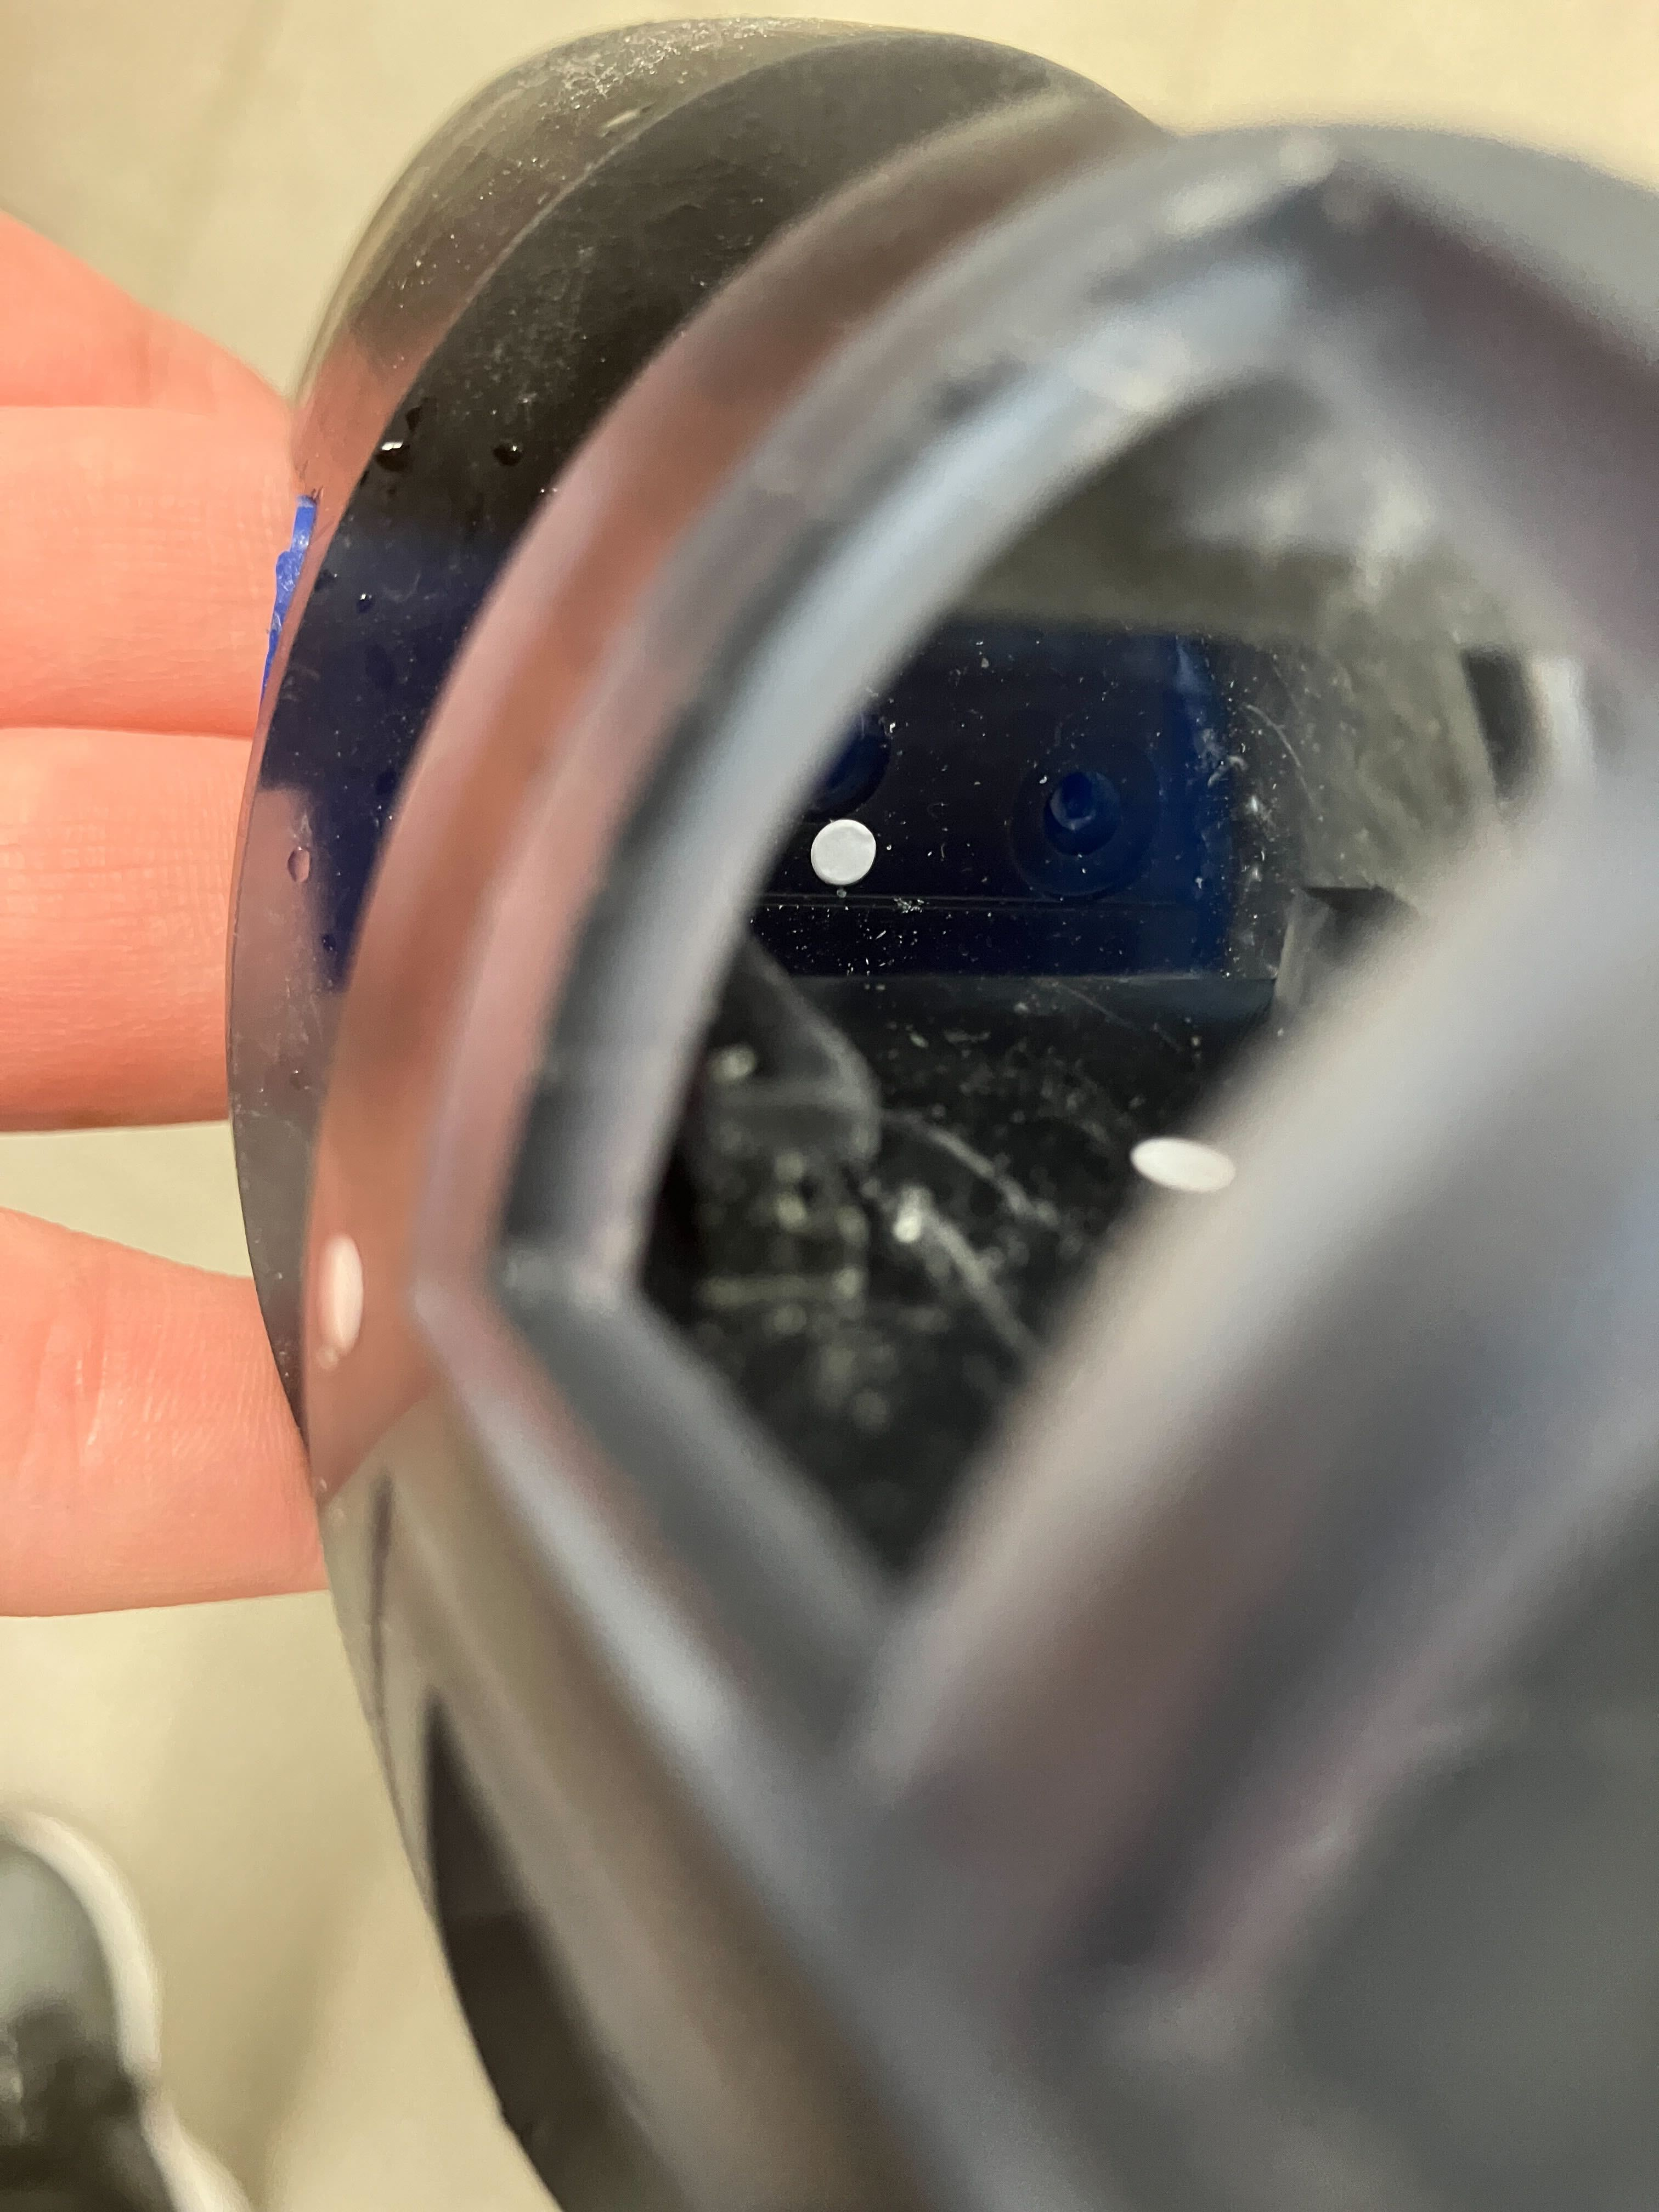
\includegraphics[width=0.8\linewidth]{chapters/picture/bousui_naka.jpg}
            \subcaption{頭部内側}
            \label{fig:toubu_uti}
        \end{minipage}
        \begin{minipage}[b]{0.31\linewidth}
            \centering
            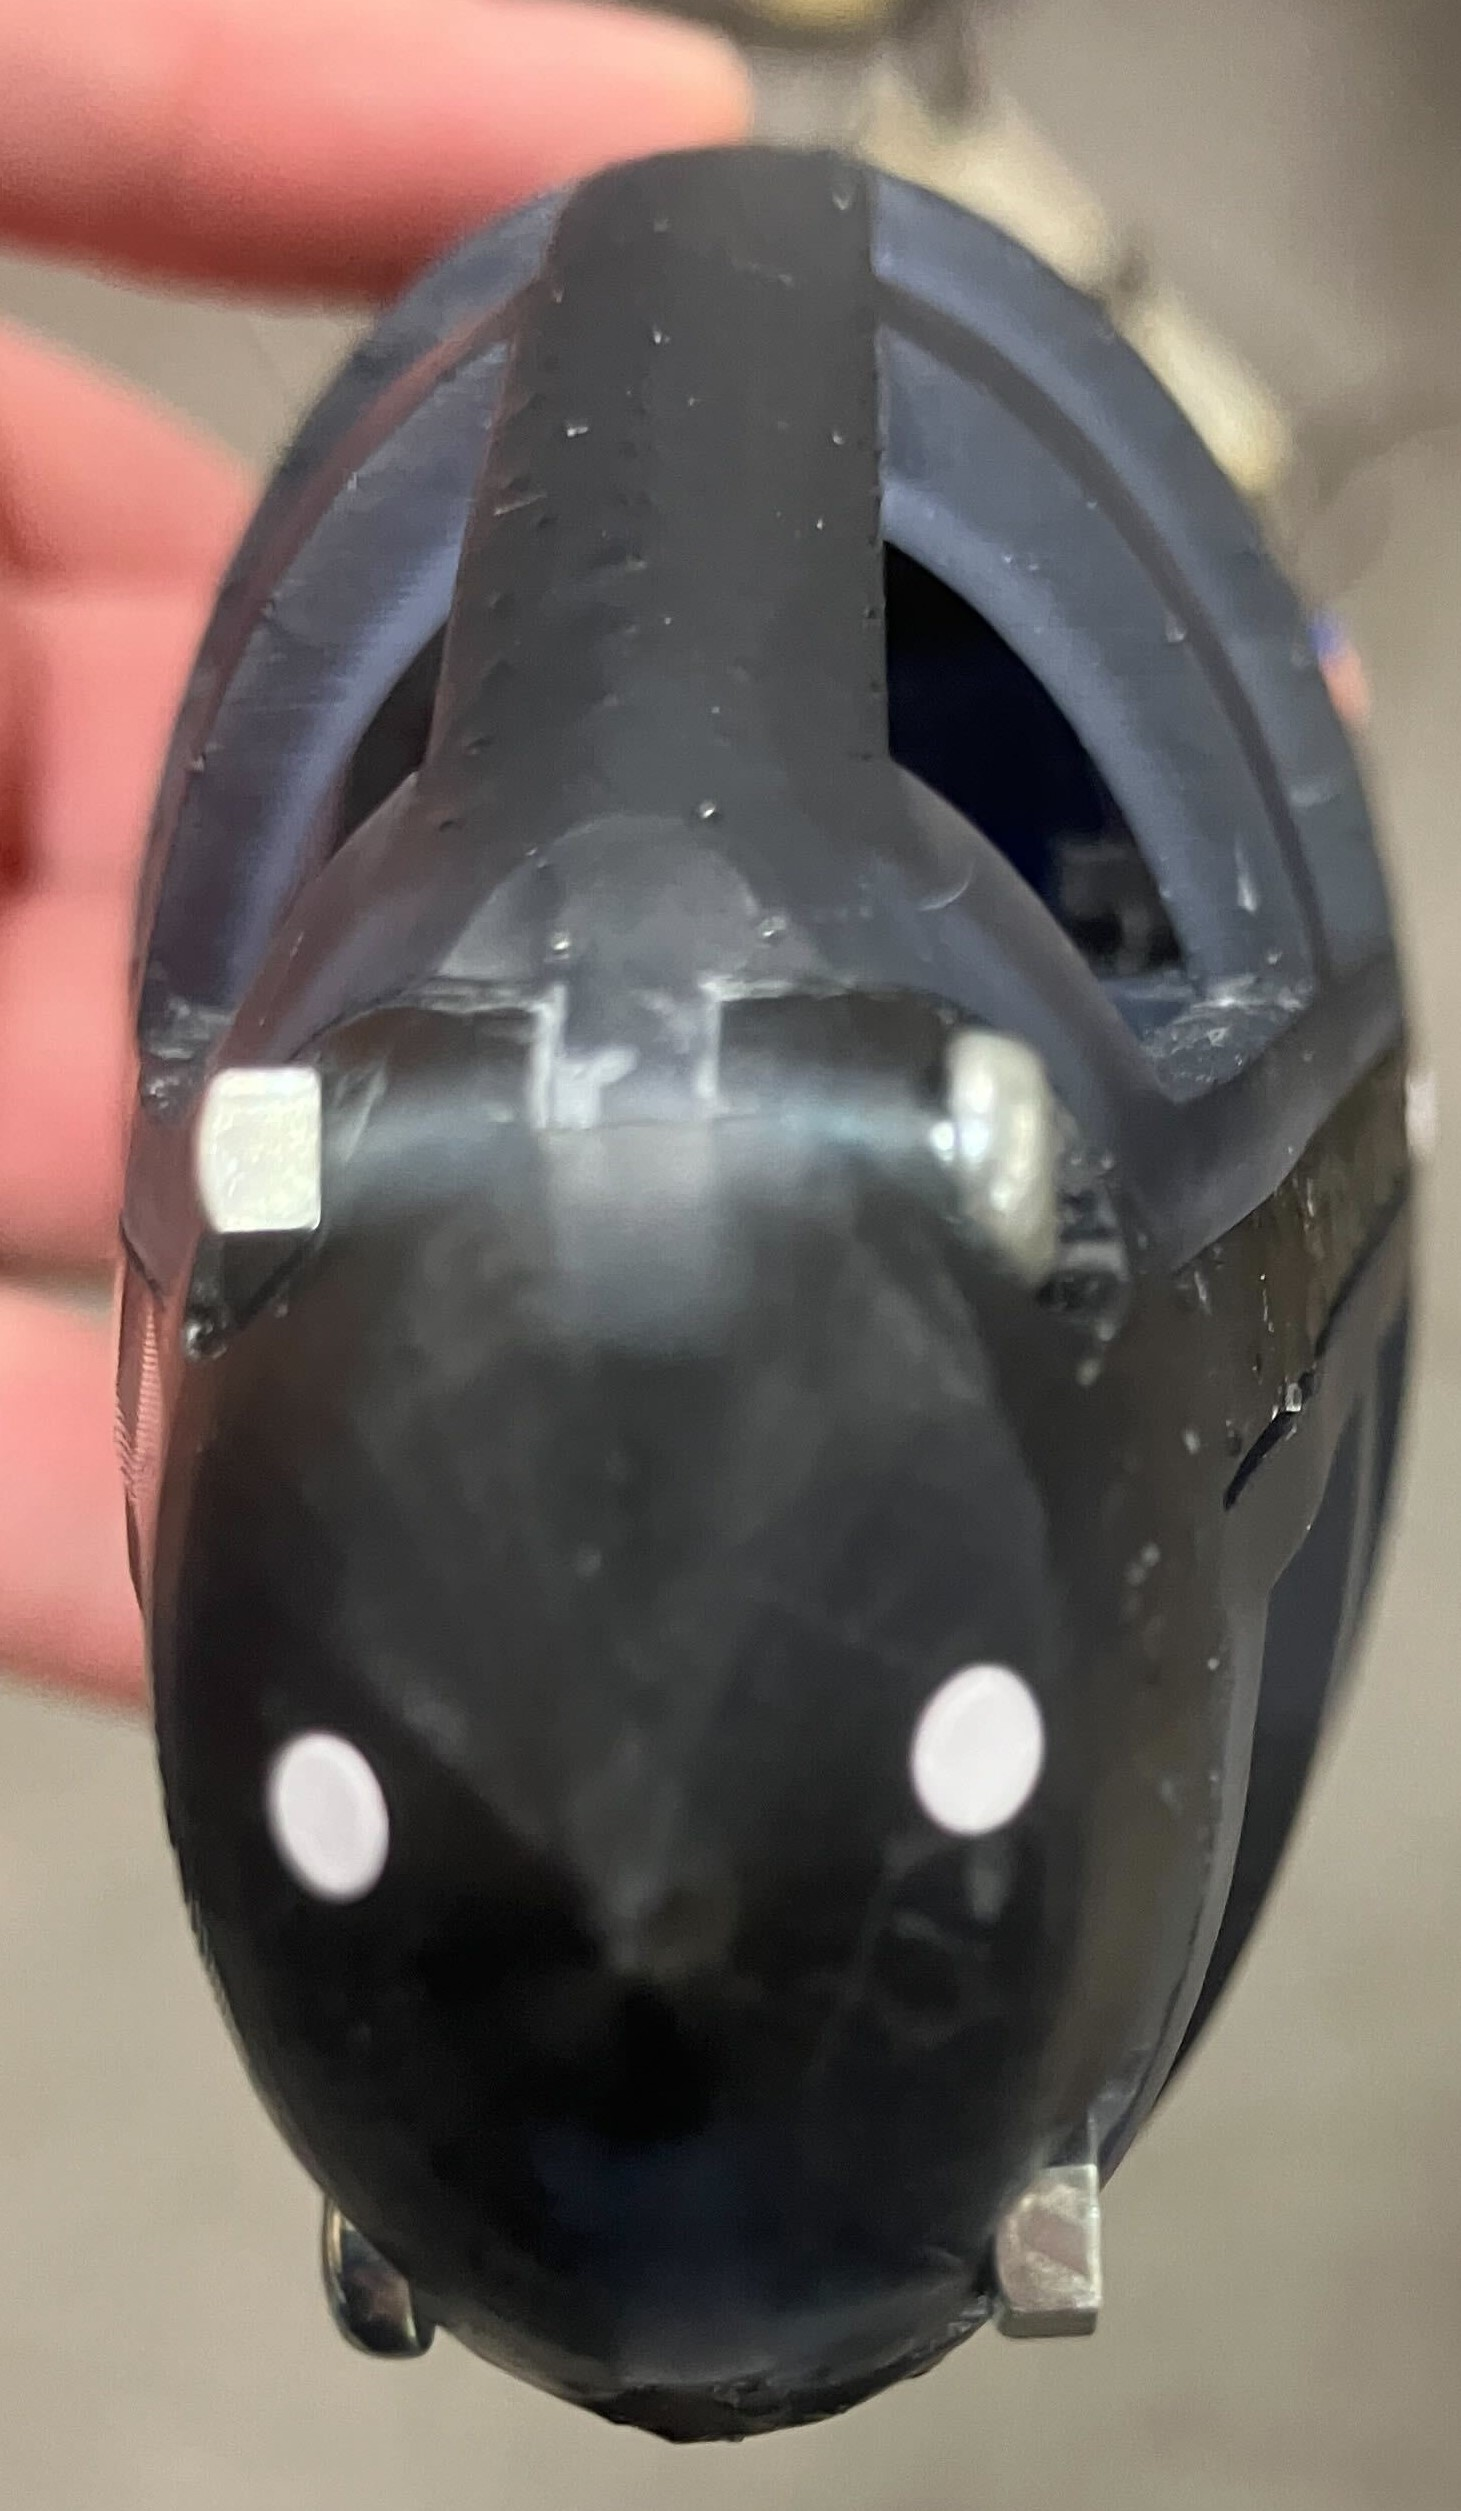
\includegraphics[width=0.7\linewidth]{chapters/picture/bousui_sentou.jpg}
            \subcaption{頭部先端}
            \label{fig:toubu_sentan}
        \end{minipage}
    \end{tabular}
    \caption{防水実験後のシールの様子}
    \label{fig:bousui_test}
\end{figure}

\newpage
また,頭部は上部と下部のカバーが開くようになっており,メンテナンス性向上のためにねじ止めではなくワンタッチでカバーを開閉できるようにしている
(図\ref{fig:head_open},\ref{fig:rock}).
それに加えて制御回路とバッテリーを取り出しやすくするためにねじで固定するのではなく,図\ref{fig:toubu_kiban},図\ref{fig:toubu_battery}のように溝にはめストッパーをつける
ことで頭部に配置している.

\begin{figure}[t]
    \centering
    \begin{minipage}[b]{0.3\linewidth}
        \centering
        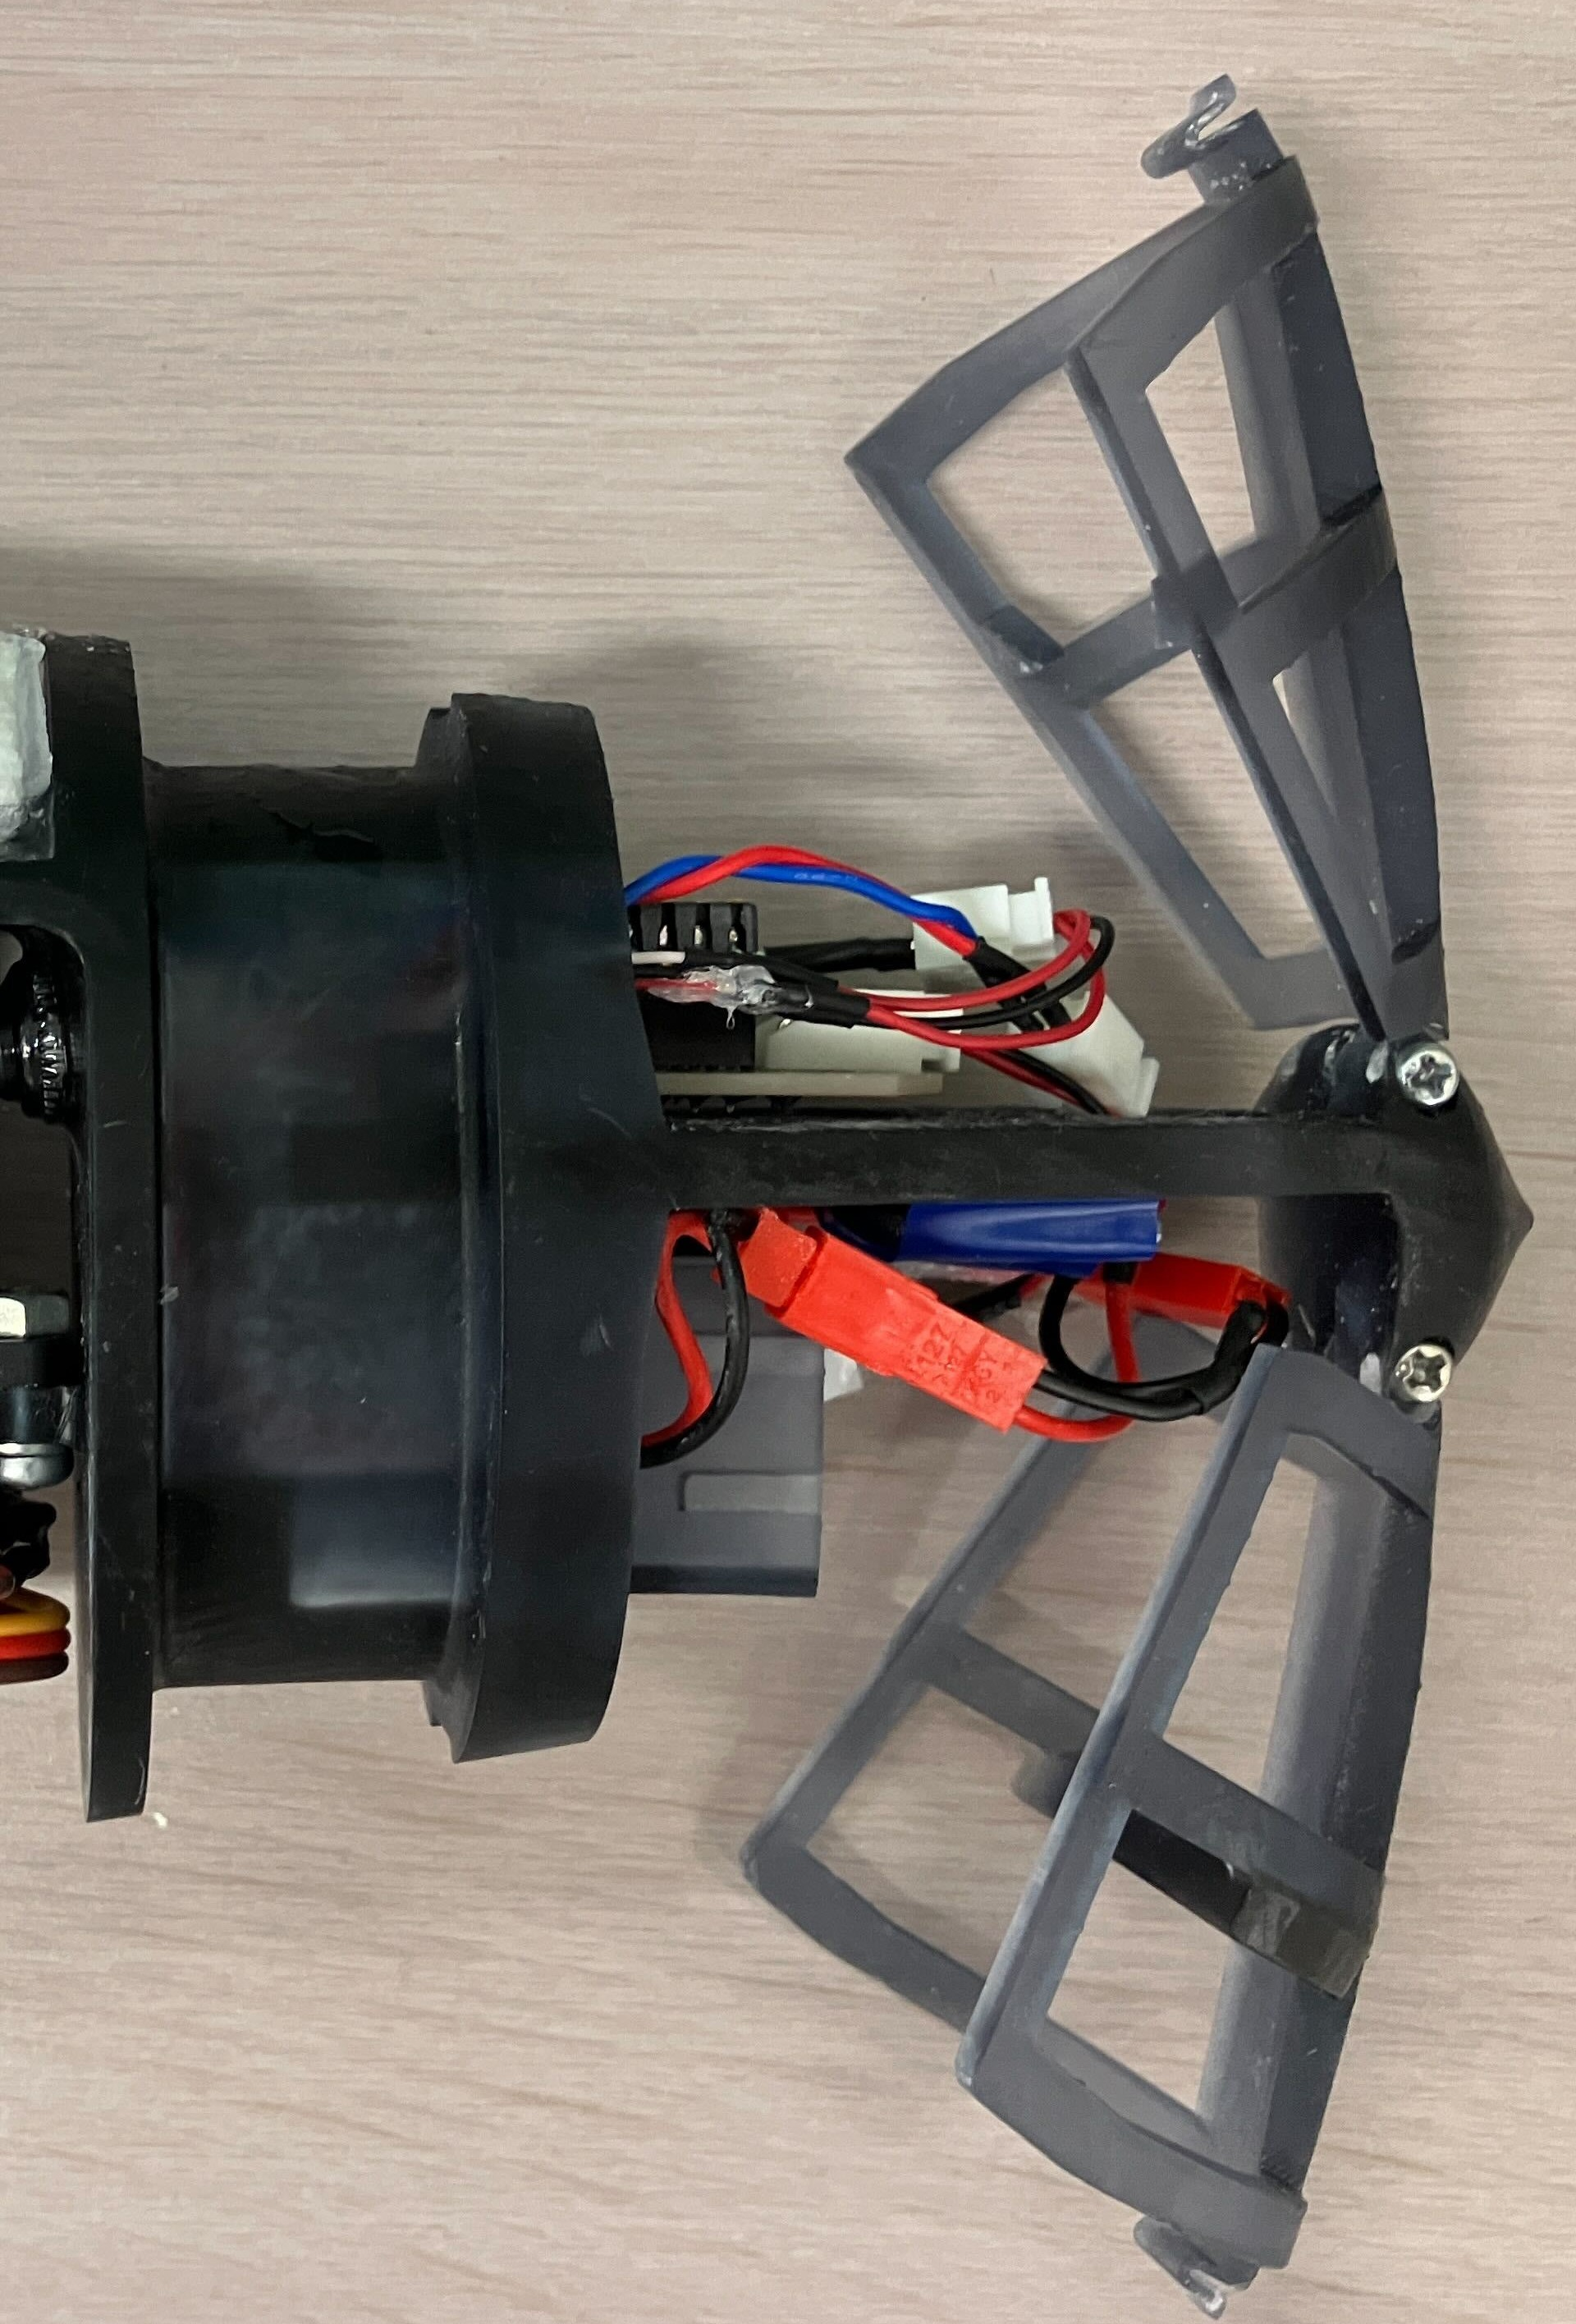
\includegraphics[width=0.6\linewidth]{chapters/picture/open_head.jpg}
        \caption{頭部開放時の様子}
        \label{fig:head_open}
    \end{minipage}
    \begin{minipage}[b]{0.5\linewidth}
        \centering
        \setPicture{rock.png}
        \caption{ワンタッチロックの仕組み}
        \label{fig:rock}
    \end{minipage}
\end{figure}
\begin{figure}[t]
    \centering
    \begin{minipage}[b]{0.4\linewidth}
        \centering
        \setPicture{toubu_kiban.png}
        \caption{基板固定方法}
        \label{fig:toubu_kiban}
    \end{minipage}
    \hspace{0.1\linewidth}
    \begin{minipage}[b]{0.4\linewidth}
        \centering
        \setPicture{toubu_battery.png}
        \caption{バッテリー固定方法}
        \label{fig:toubu_battery}
    \end{minipage}
\end{figure}

\subsubsection{胴体部}
胴体部は細かく分けて駆動部,弾性体部,尾びれ部で構成されている.
駆動部は頭部と一体化しており,試作機と同じサーボモータを配置し,プーリー(PLA樹脂)を取り付けている.また,サーボモータの信号線を制御回路側につなげるために防水キャプコン
(オーム電機,OA-WS04M-20/25)を配置し,さらに電源スイッチも配置している.また,駆動部にはカバーをかぶせ魚らしい形状になるようにしている.



弾性体部は弾性体(ポリプロピレン板,厚さ0.75 mm)と骨格リンク(PLA樹脂),ワイヤ(ポリエステル製,0.40 mm)で構成している.骨格リンクは厚みを6mmで作製し,14 mm間隔を空
けながら配置した.リンクには図のようにワイヤを通すために2 mmの穴を4 カ所開けており,さらに胴体内部を浸水させるために大きめの穴を6 個開けている.また,リンクと弾性体は
ネジを用いて二点止めし,外皮の動きがリンクの固定状態に影響を与えないようにした.

